% This work is licensed under the Creative Commons Attribution-NonCommercial 4.0 International License.
% To view a copy of this license, visit http://creativecommons.org/licenses/by-nc/4.0/
% or send a letter to Creative Commons, PO Box 1866, Mountain View, CA 94042, USA.

% !TEX TS-program = xelatex

\documentclass[../Main/chem371-notes.tex]{subfiles}

\setcounter{chapter}{9}
\begin{document}

\chapter{Intermolecular interactions and solvation}

All our discussions have so far centered on molecules in the gas phase.
In this chapter we will look at how to compute weak interactions between different molecules (intermolecular interactions) and the more general case of one molecule interacting with a large number of solvent molecules.
Due to its complexity, the problem of computing accurate thermochemical and kinetic properties in solution is still an open problem.

\section{Intermolecular interactions}

An important are of application of quantum chemistry is the prediction of change in energy when two molecules interact to form a weakly bound complex.
For example, molecules A and B could form a hydrogen bond, a polar interaction, or be bound by a weak dispersion forces to form the cluster \ce{A\cdots B}
\begin{equation}
\ce{A + B} \rightarrow \ce{A\cdots B}
\end{equation}
The interaction energy ($\Delta E_\text{int}$) for the above process is defined as the energy difference
\begin{equation}
\Delta E_\text{int} = E(A\cdots B) - E(\text{A}) - E(\text{B})
\end{equation}
and can be computed by performing three separate computations.

The interaction energy may be decomposed into a number of different physical effects that cause A and B to attract or repel.
These intermolecular interactions can be first of all divided into \emph{short-range}, which decay as exponentially with the distance $R$, $\exp(-\alpha R)$, and \emph{long-range} interactions that decay as an inverse power of $R$, $R^{-n}$.
At long-range, the main contributions to the interaction energy are \emph{electrostatic}, \emph{induction}, and \emph{dispersion} interactions.
Electrostatic interactions ($\Delta E_\text{elst}$) arise from the charge distribution of electrons in molecules.
Examples, are charge-charge interactions between ions of opposite charge (for example, \ce{Na+} and \ce{Cl-}), dipole-dipole interactions in neutral molecules (for example, two \ce{CO} molecules), quadrupole-quadrupole interactions, etc.
The presence of one or more molecules causes a a particular molecule to experience a distortion of its electric distribution causing \emph{induction effects} ($\Delta E_\text{ind}$). Since induction leads to a stabilization, its effect is always negative (and generally nonadditive).
Quantum mechanical fluctuations of the electrons also cause \emph{dispersion interactions} ($\Delta E_\text{disp}$), which tend to be weaker and attractive.

Short-range interactions arise from the overlap of the wave functions of the two molecules A and B.
The most important physical effect at short range is \emph{exchange interactions} ($\Delta E_\text{exch}$).
These are repulsive and are mostly a consequence of the electrons satisfying the Pauli principle, which prevents electrons with the same spin from occupying the same position in space.
Another short-range interaction is \emph{charge transfer} ($\Delta E_\text{CT}$), which arises when one molecule can donate and electron to another acceptor molecule.
This interaction is attractive.

\section{Symmetry-adapted perturbation theory}

The interaction energy may be decomposed into contributions from all of these physical effects
\begin{equation}
\Delta E_\text{int} = \Delta E_\text{elst} + \Delta E_\text{ind} + \Delta E_\text{disp} + \Delta E_\text{exch}+ \Delta E_\text{CT}
\end{equation}
However, a conventional quantum chemical computation on the molecules A, B, and \ce{A . . . B} does not directly decompose the interaction energy into these contributions.

Symmetry-adapted perturbation theory (SAPT) provides a way to compute the various contributions to the interaction energy.
In SAPT, one performs a DFT or wave function computation on the separate molecules A and B.
Afterwards, the interaction energy is estimate via perturbation theory.
The Hamiltonian of the \ce{A . . . B}  system is partitioned into terms that describe the molecule A ($\hat{H}_\mathrm{A} = \hat{F}_\mathrm{A} + \hat{V}_\mathrm{A} $), terms that describe B ($\hat{H}_\mathrm{B} =  \hat{F}_\mathrm{B} + \hat{V}_\mathrm{B}$), and terms that account for the interaction of A and B ($\hat{H}_\mathrm{AB}$).
This amounts to partitioning the Hamiltonian as
\begin{equation}
\hat{H} = \hat{F}_\mathrm{A} + \hat{V}_\mathrm{A} + \hat{F}_\mathrm{B} + \hat{V}_\mathrm{B} + \hat{H}_\mathrm{AB}
\end{equation}
This partitioning allows to separate the interaction energy into different contributions with different physical interpretation.
The Hamiltonian terms for each molecule are divided into a part that does not include electron correlation ($\hat{F}$) and the electron-electron interaction ($\hat{V}$).
In this way, SAPT can separate contributions to the interaction energy that arise from both intramolecular correlation and intermolecular forces.

\mfigure{
\captionof{table}{Comparison of the contributions to the interaction energy (in \kcal) in the water dimer and the methane dimer computed at the SAPT0 level. The geometry of the dimers was optimized at the B3LYP/aug-ccp-VDZ level of theory. SAPT0 computations used the aug-cc-pVDZ basis.}
%\normalsize 
\begin{tabular}{@{} lcc @{}}
\toprule
Term & \ce{H2O . . . H2O} & \ce{CH4 . . . CH4} \\
\midrule
$E_\mathrm{elst}^{(10)}$ & $-$\textbf{8.58} & $-0.10$ \\
$E_\mathrm{exch}^{(10)}$ & $+$\textbf{7.27} & $+$\textbf{0.27} \\
$E_\mathrm{ind,resp}^{(20)}$ & $-2.98$  & $-0.03$\\
$E_\mathrm{exch-ind,resp}^{(20)}$ & $+1.59$ & $+0.02$\\
$E_\mathrm{disp}^{(20)}$ & $-2.28$ & $-$\textbf{0.50} \\
$E_\mathrm{exch-disp}^{(20)}$ & $+0.42$ & $+0.03$\\
$\delta_{HF}^{(2)}$ & $-0.96$ & $-0.02$\\[3pt]
\textbf{Total} & $-5.52$ & $-0.33$\\
\bottomrule
\end{tabular}
\label{tab:solvation:sapt0}
}

In the simplest form of SAPT (SAPT0), the monomer energies are computed at the HF level and their interaction is estimated via perturbation theory.
In SAPT0 the energy is decomposed into contributions of the form $E^{(ij)}$, where $i$ indicates the order of at which the interaction is accounted for, and $j$ is the level at which correlation is treated in each molecule.
The SAPT0 interaction energy treats electron correlation on the fragment to order zero (equivalent to HF theory) while the interaction is treated at order one and two. Therefore SAPT0 contains terms of the form $E^{(i0)}$ as shown here
\begin{equation}
E_\mathrm{SAPT0} = E_\mathrm{elst}^{(10)} + E_\mathrm{exch}^{(10)} + E_\mathrm{ind,resp}^{(20)} +
E_\mathrm{exch-ind,resp}^{(20)} + E_\mathrm{disp}^{(20)} + E_\mathrm{exch-disp}^{(20)} + \delta_{HF}^{(2)}
\end{equation}
These terms are: 1) the electrostatic energy ($E_\mathrm{elst}^{(10)} $) compute from the HF density, 2) the exchange repulsion ($E_\mathrm{exch}^{(10)}$), 3) the induction energy ($E_\mathrm{ind,resp}^{(20)} $) and exchange induction ($E_\mathrm{exch-ind,resp}^{(20)}$) due to the HF density on the other molecule, 4) dispersion ($E_\mathrm{disp}^{(20)}$) and exchange dispersion ($E_\mathrm{exch-disp}^{(20)}$), and 5) higher order corrections ($\delta_{HF}^{(2)}$).

Table~\ref{tab:solvation:sapt0} reports results from a SAPT0 computation of the interaction energy for the water dimer and methane dimer.
SAPT0 predicts that the hydrogen bond stabilizes the water dimer by $-$5.52 \kcal, with large contributions from electrostatic interactions, induction, and dispersion.
In the case of the methane dimer, electrostatic effects play a minor role, and the weak interaction energy ($-$0.33 \kcal) is dominated by dispersion and exchange contributions.
More accurate versions of SAPT include SAPT2 and several variants of SAPT2 with improved descriptions of dispersion, electrostatic interactions, and exchange terms.

\section{Modeling reactions in solutions}

\mfigure{
\centering{
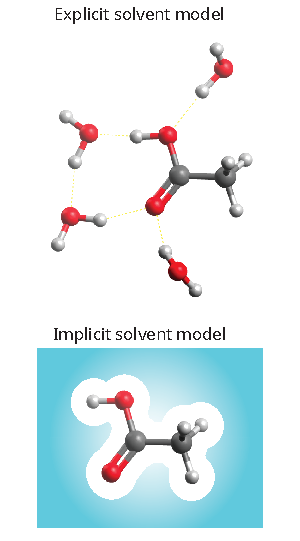
\includegraphics[width=2.00in]{img/solvation.png}
}
\captionof{figure}{Explicit solvent models include a small number of solvent molecules around the solute. Implicit solvent models account for the presence of a solvent with a continuum that interacts with the solute.}
\label{fig:solvent:implicit_explicit}
}

%The interaction of a solute with solvent molecules 
Modeling reactions in solutions is a problem related to that of computing intermolecular interactions; however, it is significantly more complex due to the fact that in principle one should sample over all possible arrangements of the solvent around a solute that are energetically accessible at a given temperature $T$.
The computation of a reaction in solution can be, however, broken into simple steps.
For example, the pK$_\mathrm{a}$ of an acid HA, which is related to the free energy of the following reaction 
\begin{equation}
\ce{HA_{(aq)}} \rightarrow \ce{H^+_{(aq)}} + \ce{A^-_{(aq)}}, \quad 
\end{equation}
via $pK_\mathrm{a} = \Delta G_\textrm{aq} / RL \ln(10)$, can be obtained via a thermodynamic cycle  that breaks the free energy computation in three steps
\begin{center}
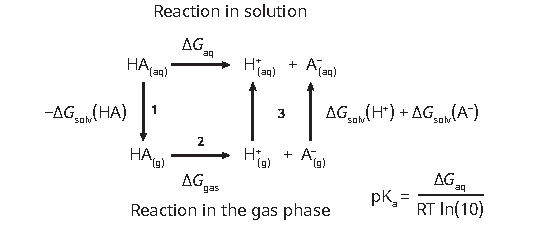
\includegraphics[width=4.0in]{img/solvent.pdf}
\end{center}
In the first step, the acid in solution is brought in the gas phase, giving a free energy contribution equal to the negative of the solvation energy of HA.
In the second step, the acid dissociates into \ce{H+} + \ce{A-}, with corresponding free energy change equal to the free energy of dissociation ($\Delta G_\textrm{gas}$).
In the third step, the \ce{H+} + \ce{A-} ions are solvated.
This cycle allows to compute $\Delta G_\textrm{aq}$ as
\begin{equation}
\Delta G_\textrm{aq} = \Delta G_\textrm{gas} + \Delta G_\textrm{solv}(\ce{H^+}) + \Delta G_\textrm{solv}(\ce{A^-})  -\Delta G_\textrm{solv}(HA)
\end{equation}
Of these three free energy contribution, $\Delta G_\textrm{gas}$ can be computed directly with quantum chemistry methods.

Computing the solvation free energies requires modeling the interaction of the solute with solvent molecules (in this case water).
In solutions, the solvent molecules can interact with the solute in many ways, and therefore it is also necessary to potentially sample a large number of solute-solvent geometries.
There are two main strategies for introducing the effect of solvents in quantum mechanical computations: explicit and implicit models (see Fig.~\ref{fig:solvent:implicit_explicit}).
In \emph{explicit solvent models}, the solute is surrounded by a small cluster of solvent molecules that captures the main interactions due to the first solvation shell.
However, a cluster model is often insufficient to accurately model solvation because if the cluster is too small it neglects important long-range interactions.
\emph{Implicit solvent models} model the effect of a solvent with a cavity surrounded by a continuum that responds to the presence of the solute. This continuum exerts an additional potential on the electrons of the solute that depends on the electron density of the solute.
Therefore, the effect of the solvent modeled by implicit models requires a self-consistent optimization that is performed together with the Hartree--Fock or DFT SCF steps.

\section{Polarizable continuum models}

\mfigure{
\centering{
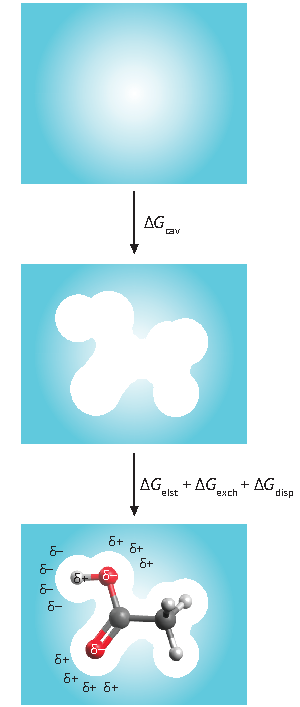
\includegraphics[width=2.00in]{img/pcm.png}
}
\captionof{figure}{Explicit solvent models include a small number of solvent molecules around the solute. Implicit solvent models account for the presence of a solvent with a continuum that interacts with the solute.}
\label{fig:solvent:pcm}
}

The most widely used implicit solvation models are based on Tomasi's polarizable continuum model (PCM).
In PCM, the solute is surrounded by a cavity built by taking the union of spheres centered on each of the atoms.
There are two variants of PCM: a dielectric PCM (or simple PCM), which models a cavity surrounded by a polarizable medium, and the conductor PCM (C-PCM), in which the medium is a conductor-like material.
The dielectric PCM is what you will typically run when modeling solvent effects.

The solvation free energy may be decomposed into four physical contributions
\begin{equation}
\Delta G_\mathrm{solv}= \Delta G_\mathrm{elst} + \Delta G_\mathrm{exch} + \Delta G_\mathrm{disp} + \Delta G_\mathrm{cav}
\end{equation}
where the first three correspond to electrostatic, exchange, and dispersion interactions of the solute with the solvent, while $\Delta G_\mathrm{cav}$ is the free energy associated with forming a cavity in the solvent.
This process is broken down into two steps in Fig.~\ref{fig:solvent:pcm}.
In the first step a cavity is formed in the solvent, which requires an amount of free energy equal to $\Delta G_\mathrm{cav}$.
In the second step, a molecule is placed in the cavity and the solvent interacts with the solute leading to electrostatic, exchange, and dispersion interactions.

The PCM model includes the response of the solvent due to the distribution of charges in the solute, and therefore, \emph{it accounts only for the electrostatic interaction}.
Since the PCM only affects the electronic energy, it introduces a shift in the total energy ($\Delta E_\mathrm{elst}$).
Obtaining the corresponding free energy change requires a vibrational analysis to compute corrections due to the free energy change.
In many cases this is a good approximation to the solute-solvent interaction.
However, if exchange and dispersion effects dominate the solute-solvent interactions, then the PCM method cannot accurately predict the solvation free energy.
To estimate the free energy of cavitation, a model of the solvent is required in addition to the PCM method.

In the dielectric PCM, different solvents are characterized by the relative permittivity $\epsilon_r$ (also called the dielectric constant), which is a measure of the electric polarizability of the dielectric continuum. The permittivity is related to molecular polarity and for polar molecules like water it is as high as 78.4, while for less polar molecules it decreases (acetonitrile = 37.5, ethanol = 24.3), and becomes almost equal to one for nonpolar solvents (benzene = 2.3).
%Outside the cavity, PCM models a general dielectric medium with dielectric constant $\epsilon$.
%Variants of PCM exist that can use a conductor-like approximation to the dielectric medium.


\end{document}